
%  Verwendete Plattform /Software (Installationshinweise, Versionen)
% Schnittstellenbeschreibung des Web Services (WSDL/WADL/Swagger, …​)
% Umsetzung, Technologien, Sicherheitskonzepte, API

\section{Technologien}


\subsection{Architektur}

%Beschriebender Text?

\begin{figure}[H]
	\hspace{-1.5cm}
	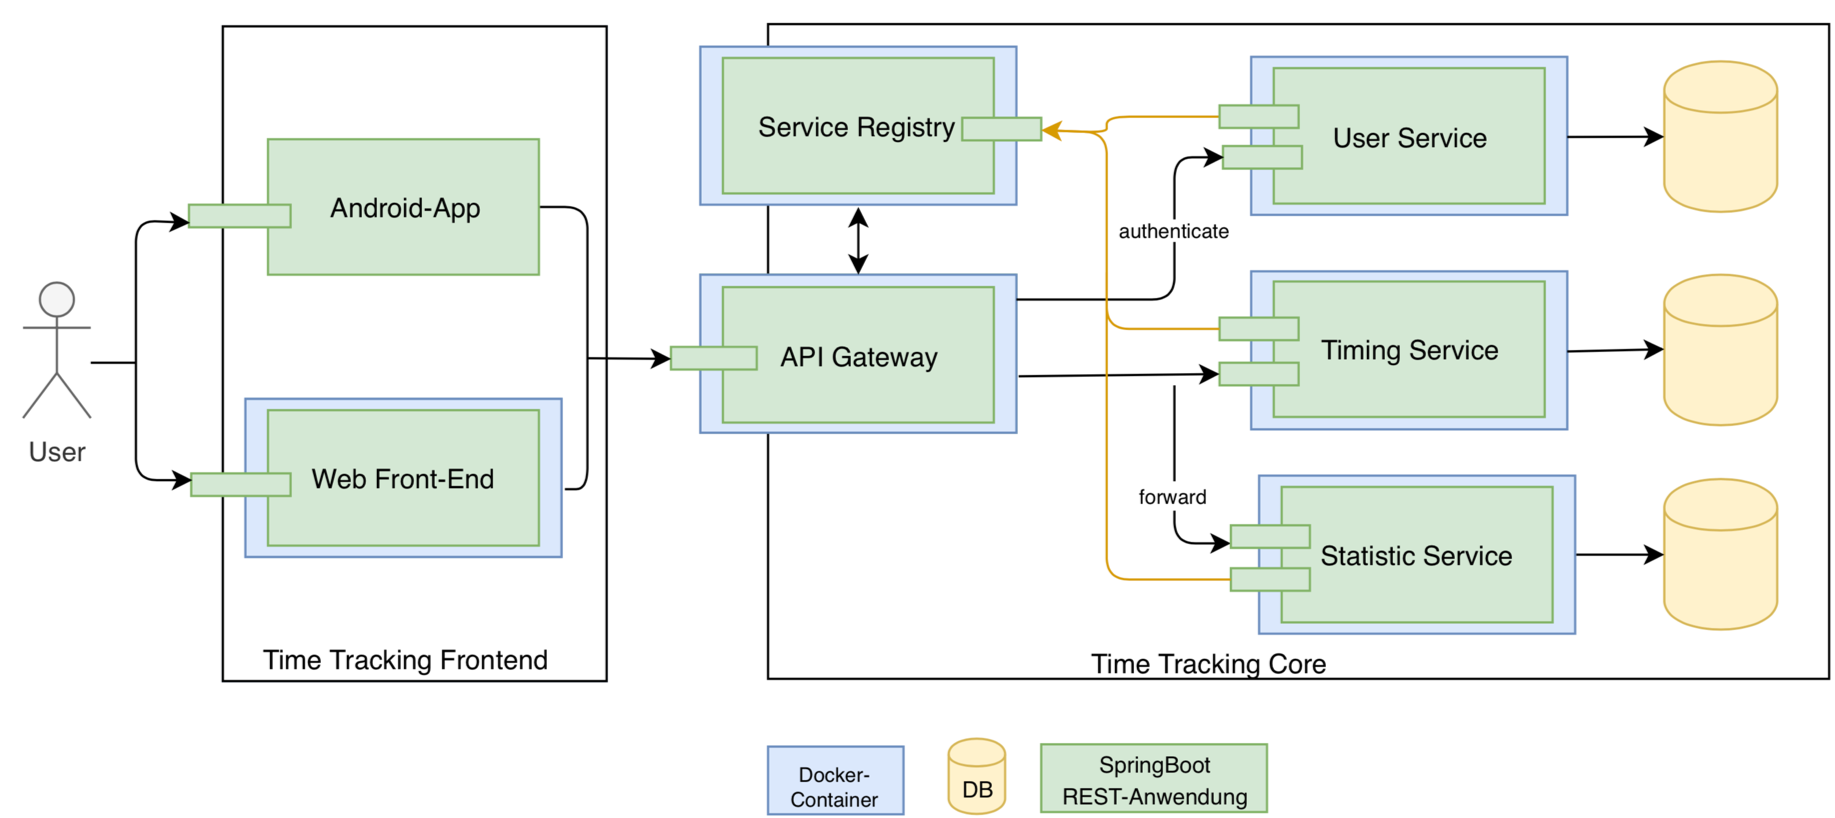
\includegraphics[width=1.15\linewidth]{SCC_Architecture-99final.png}
	\caption{Architektur von TimeTracker}
	\label{fig:Architektur}
\end{figure}

Anmerkung: Die Andoid-App wurde nicht im Rahmen der Lehrveranstaltung fertig gestellt und ist somit noch ausstehend. 

\subsection{Übersicht verwendeter Technologien}
% Tabelle 
\renewcommand{\arraystretch}{1.3} % Für die Abstände zwischen den Spalten 
\begin{table}[H] 
	% \small
	\centering
	\caption{Technologien}
	\begin{tabularx}{\textwidth}{l|c|X}
		\textbf{Name} & \textbf{Version} & \textbf{Verwendung} \\
		\hline
		Java & JDK 1.8.0 & Verwendete Programmiersprache \\
		Mavent & 3.1.0  & Build-Management-Tool \\
		Spring boot & 2.0.2 & Java Framework für Web-Systeme \\
		MySQL & 5.7.0 & Relationale Datenbank \\
		Netflix Zuul & 1.3.1 & Edge Service für dynamisches Routen, \newline Monitoring und Sicherheit  \\
		Netflix Eureka & 1.9.2 & REST-basierter Service,  Zuordnen von Services   \\
		JSON & - & Dateiformat bei Übermittlung \\
		REST & - & Programmierparadigma für Webservices \\
		React & 16.1.1 & JavaScript Bibliothek für User Interfaces  \\
		single-spa & 2.6.0 & JavaScript Framework für Front-End Microservices \\
		OpenAPI  (Swagger) & 3.0. & REST-Schnittstelle basiert auf Standard von OpenAPI,  Zum Entwerfen und Dokumentieren der RESTfull-Schnittellen wurde das Framework Swagger verwendet \\
		Postman & 6.5.3 & API Development Environment \\
		Docker & 18.09.0 & Umgebung für Container \\
	\end{tabularx}
	\label{tab:Technologien}
\end{table}

\subsection{Schnittstellenbeschreibung}
% Links von Server mit http://editor.swagger.io/ oder https://swagger.io/tools/swagger-inspector/ or https://swagger.io/tools/swagger-ui/

Die API wurde nach dem OpenAPI-Standard entwickelt und generierte automatisch ein Controller in Java. Eine Auflistung aller Methoden ist über die folgenden Links zu erreichen. Zusätzlich befindet sich im Anhang (Seite \pageref{Anhang}) ein Ausdruck der automatisch generierten Dokumentation.

\begin{itemize}
	\item frontend-service: 
	\item timing-service: 
	\item user-service:
\end{itemize}

\subsection{Sicherheit}

Die Sicherheit wurde mittels \textbf{JSON Web Token (JWT)} und umgesetzt. Dabei erhält der Benutzer beim Login eine UUID, mittels derer er sich gegenüber den Diensten authentifizieren kann. 

Des weiteren wird die Sicherheit der Verbindung mittels der Transportverschlüsselung \textbf{HTTPS} gewährleistet. 

